% questions.tex —— 2020 年·天津卷 · 题目内容片段（无答案）
% 由 tools/generate_projects.py 依来源总账自 2020/2020_数学真题_天津_试题.md 生成，勿手改（改源 MD 后重跑）


\begin{gknotice}
\textbf{来源说明}：本题面依据固定源 PDF 的两页 A3 题面逐题转录，原卷印刷页码为 1131、1132。第 1131 面为选择题 1—9、填空题 10—15 与解答题 16、17；第 1132 面为解答题 18—20。全卷三处节头依次为「一、选择题」「二、填空题」「三、解答题」，题号与索引一致；所有数值、分式、根号与上下标均回原页 300—600 dpi 核对。

\textbf{解析归属}：固定源不附答案或解析；配套答案与解析均由本库按本题面独立复算（等级 D，非官方）。

\textbf{图形说明}：第 3 题的四个函数图象选项、第 4 题的频率分布直方图、第 15 题的四边形与第 17 题的三棱柱，均由项目内 TikZ 矢量源按原页几何重绘；其余各题原页无图。
\end{gknotice}

\gkpart{一、选择题}

\begin{question}
\gkti{1}设全集 $U=\{-3,-2,-1,0,1,2,3\}$，集合 $A=\{-1,0,1,2\}$，$B=\{-3,0,2,3\}$，则 $A\cap(\complement_UB)=$\mbox{（　　）}

（A）$\{-3,3\}$；（B）$\{0,2\}$；（C）$\{-1,1\}$；（D）$\{-3,-2,-1,1,3\}$。

\end{question}
\begin{question}
\gkti{2}设 $a\in\mathbf R$，则「$a>1$」是「$a^2>a$」的\mbox{（　　）}

（A）充分不必要条件；（B）必要不充分条件；（C）充要条件；（D）既不充分也不必要条件。

\Needspace{0.4\textheight}
\end{question}
\begin{question}
\gkti{3}函数 $y=\dfrac{4x}{x^2+1}$ 的图象大致为\mbox{（　　）}
\nopagebreak[4]
\begin{center}% 2020 天津卷 第 3 题：函数 y = 4x/(x^2+1) 的四个图象选项（2×2 四联图）
% 来源 PDF：普通高考/2020/2020天津.pdf 第 1 页（A3 横排），印面 1131，第 3 题题干下方
% 逐格核对原页矢量曲线（600 dpi 渲染并读 SVG 路径，单位 pt）后确认四幅互不相同：
%   (A) 奇函数；x 轴刻度 1 处取最大值 2（曲线最高点横坐标与刻度 1 重合），
%       x=-1 处取最小值 -2，两端趋于 0 —— 即 y=4x/(x^2+1)；
%   (B) 与 (A) 关于 x 轴对称，最大值在 x=-1，最小值在 x=1 —— 即 y=-4x/(x^2+1)；
%   (C) 偶函数；x=±1 处各取最大值 2，原点处为尖点且函数值为 0 —— 即 y=4|x|/(x^2+1)；
%   (D) 与 (C) 关于 x 轴对称，x=±1 处各取最小值 -2 —— 即 y=-4|x|/(x^2+1)。
% 原页每幅图均画：x 轴（右端箭头、标 x）、y 轴（上端箭头、标 y）、原点 O、
%   x 轴刻度 1、y 轴刻度 2；坐标轴在 x 方向总长约 13.6 个单位，曲线自 -6.5 画到 6.5。
\begin{tikzpicture}[font=\small,>=Stealth,line cap=round,line join=round]
  % (A) 左上：y = 4x/(x^2+1)
  \begin{scope}[shift={(0,3.05)},x=0.32cm,y=0.42cm]
    \draw[->] (-6.9,0)--(7.0,0) node[below,inner sep=2pt] {$x$};
    \draw[->] (0,-2.5)--(0,3.05) node[left,inner sep=2pt] {$y$};
    \node[below left,inner sep=1pt] at (0,0) {$O$};
    \draw (1,0.12)--(1,-0.12) node[below,inner sep=6pt] {$1$};
    \draw (0.24,2)--(-0.30,2);
    \node[above left,inner sep=2pt] at (-0.32,2) {$2$};
    \draw[line width=0.9pt,domain=-6.5:6.5,samples=300,smooth]
      plot (\x,{4*\x/(\x*\x+1)});
    \node at (-5.6,-3.35) {(A)};
  \end{scope}
  % (B) 右上：y = -4x/(x^2+1)
  \begin{scope}[shift={(4.65,3.05)},x=0.32cm,y=0.42cm]
    \draw[->] (-6.9,0)--(7.0,0) node[below,inner sep=2pt] {$x$};
    \draw[->] (0,-2.5)--(0,3.05) node[left,inner sep=2pt] {$y$};
    \node[below left,inner sep=1pt] at (0,0) {$O$};
    \draw (1,0.12)--(1,-0.12) node[below,inner sep=6pt] {$1$};
    \draw (0.24,2)--(-0.30,2);
    \node[above left,inner sep=2pt] at (-0.32,2) {$2$};
    \draw[line width=0.9pt,domain=-6.5:6.5,samples=300,smooth]
      plot (\x,{-4*\x/(\x*\x+1)});
    \node at (-5.6,-3.35) {(B)};
  \end{scope}
  % (C) 左下：y = 4|x|/(x^2+1)
  \begin{scope}[shift={(0,0.30)},x=0.32cm,y=0.42cm]
    \draw[->] (-6.9,0)--(7.0,0) node[below,inner sep=2pt] {$x$};
    \draw[->] (0,-2.5)--(0,3.05) node[left,inner sep=2pt] {$y$};
    \node[below left,inner sep=1pt] at (0,0) {$O$};
    \draw (1,0.12)--(1,-0.12) node[below,inner sep=6pt] {$1$};
    \draw (0.24,2)--(-0.30,2);
    \node[above left,inner sep=2pt] at (-0.32,2) {$2$};
    \draw[line width=0.9pt,domain=-6.5:0,samples=160,smooth]
      plot (\x,{4*abs(\x)/(\x*\x+1)});
    \draw[line width=0.9pt,domain=0:6.5,samples=160,smooth]
      plot (\x,{4*abs(\x)/(\x*\x+1)});
    \node at (-5.6,-3.35) {(C)};
  \end{scope}
  % (D) 右下：y = -4|x|/(x^2+1)
  \begin{scope}[shift={(4.65,0.30)},x=0.32cm,y=0.42cm]
    \draw[->] (-6.9,0)--(7.0,0) node[below,inner sep=2pt] {$x$};
    \draw[->] (0,-2.5)--(0,3.05) node[left,inner sep=2pt] {$y$};
    \node[below left,inner sep=1pt] at (0,0) {$O$};
    \draw (1,0.12)--(1,-0.12) node[below,inner sep=6pt] {$1$};
    \draw (0.24,2)--(-0.30,2);
    \node[above left,inner sep=2pt] at (-0.32,2) {$2$};
    \draw[line width=0.9pt,domain=-6.5:0,samples=160,smooth]
      plot (\x,{-4*abs(\x)/(\x*\x+1)});
    \draw[line width=0.9pt,domain=0:6.5,samples=160,smooth]
      plot (\x,{-4*abs(\x)/(\x*\x+1)});
    \node at (-5.6,-3.35) {(D)};
  \end{scope}
\end{tikzpicture}
\end{center}
\nopagebreak[4]
\Needspace{0.4\textheight}
\end{question}
\begin{question}
\gkti{4}从一批零件中抽取 $80$ 个，测量其直径（单位：mm），将所得数据分为 $9$ 组：$[5.31,5.33)$，$[5.33,5.35)$，$\cdots$，$[5.45,5.47)$，$[5.47,5.49]$，并整理得到如下频率分布直方图，则在被抽取的零件中，直径落在区间 $[5.43,5.47)$ 内的个数为\mbox{（　　）}
\nopagebreak[4]
\begin{center}% 2020 天津卷 第 4 题：频率分布直方图
% 来源 PDF：普通高考/2020/2020天津.pdf 第 1 页（A3 横排），印面 1131，第 4 题题干下方
% 几何按原页矢量数据换算：9 个等宽组 [5.31,5.33) … [5.47,5.49]，
%   矩形高度（频率/组距）依次为 1.25、3.75、2.50、7.50、10.00、8.75、6.25、5.00、5.00，
%   组距 0.02，故各矩形面积（频率）依次为 0.025、0.075、0.05、0.15、0.20、0.175、0.125、0.10、0.10，
%   合计 1.00，与 80 个样本一致。
% 纵轴虚线只标 1.25 的整数倍刻度，自 1.25 起至 10.00（原页即 8 条虚线）；
% 横轴自 5.31 起每 0.02 标一组端点，末尾 5.49；原点左侧有断裂符号，0 标在断裂符号之外。
\begin{tikzpicture}[font=\small,
  x=0.60cm, y=0.26cm, line cap=round, line join=round]
  % 坐标轴（左端留出断裂符号与 0 的位置）
  \draw[->] (-1.35,0)--(10.35,0) node[right,inner sep=4pt] {直径/mm};
  \draw[->] (0,0)--(0,11.6) node[above,inner sep=4pt] {$\dfrac{\text{频率}}{\text{组距}}$};
  % 断裂符号
  \draw (-0.78,0.10)--(-0.36,-0.34) (-0.78,-0.34)--(-0.36,0.10);
  \node[below,inner sep=4pt] at (-1.18,0) {$0$};
  % 纵向虚线刻度 1.25—10.00
  \foreach \h/\lab in {1.25/1.25,2.50/2.50,3.75/3.75,5.00/5.00,
                       6.25/6.25,7.50/7.50,8.75/8.75,10.00/10.00}{
    \draw[dashed,line width=0.4pt] (0,\h)--(9,\h);
    \draw (-0.14,\h)--(0,\h);
    \node[left,inner sep=2pt,font=\scriptsize] at (-0.12,\h) {\lab};
  }
  % 9 个矩形
  \foreach \i/\h in {0/1.25,1/3.75,2/2.50,3/7.50,4/10.00,5/8.75,6/6.25,7/5.00,8/5.00}{
    \draw[line width=0.6pt] (\i,0) rectangle (\i+1,\h);
  }
  % 横轴刻度与标签
  \foreach \i/\lab in {0/5.31,1/5.33,2/5.35,3/5.37,4/5.39,5/5.41,
                       6/5.43,7/5.45,8/5.47,9/5.49}{
    \draw (\i,0)--(\i,-0.28);
    \node[below,inner sep=2pt,font=\scriptsize] at (\i,0) {\lab};
  }
\end{tikzpicture}
\end{center}
\nopagebreak[4]
（A）$10$；（B）$18$；（C）$20$；（D）$36$。

\end{question}
\begin{question}
\gkti{5}若棱长为 $2\sqrt3$ 的正方体的顶点都在同一球面上，则该球的表面积为\mbox{（　　）}

（A）$12\pi$；（B）$24\pi$；（C）$36\pi$；（D）$144\pi$。

\end{question}
\begin{question}
\gkti{6}设 $a=3^{0.7}$，$b=\left(\dfrac13\right)^{-0.8}$，$c=\log_{0.7}0.8$，则 $a$，$b$，$c$ 的大小关系为\mbox{（　　）}

（A）$a<b<c$；（B）$b<a<c$；（C）$b<c<a$；（D）$c<a<b$。

\end{question}
\begin{question}
\gkti{7}设双曲线 $C$ 的方程为 $\dfrac{x^2}{a^2}-\dfrac{y^2}{b^2}=1$（$a>0$，$b>0$），过抛物线 $y^2=4x$ 的焦点和点 $(0,b)$ 的直线为 $l$。若 $C$ 的一条渐近线与 $l$ 平行，另一条渐近线与 $l$ 垂直，则双曲线 $C$ 的方程为\mbox{（　　）}

（A）$\dfrac{x^2}{4}-\dfrac{y^2}{4}=1$；（B）$x^2-\dfrac{y^2}{4}=1$；（C）$\dfrac{x^2}{4}-y^2=1$；（D）$x^2-y^2=1$。

\end{question}
\begin{question}
\gkti{8}已知函数 $f(x)=\sin\left(x+\dfrac\pi3\right)$。给出下列结论：

① $f(x)$ 的最小正周期为 $2\pi$；

② $f\left(\dfrac\pi2\right)$ 是 $f(x)$ 的最大值；

③ 把函数 $y=\sin x$ 的图象上所有点向左平移 $\dfrac\pi3$ 个单位长度，可得到函数 $y=f(x)$ 的图象。

其中所有正确结论的序号是\mbox{（　　）}

（A）①；（B）①③；（C）②③；（D）①②③。

\end{question}
\begin{question}
\gkti{9}已知函数 $f(x)=\begin{cases}x^3,&x\geqslant0,\\-x,&x<0.\end{cases}$ 若函数 $g(x)=f(x)-|kx^2-2x|$（$k\in\mathbf R$）恰有 $4$ 个零点，则 $k$ 的取值范围是\mbox{（　　）}

（A）$\left(-\infty,-\dfrac12\right)\cup\left(2\sqrt2,+\infty\right)$；（B）$\left(-\infty,-\dfrac12\right)\cup\left(0,2\sqrt2\right)$；（C）$(-\infty,0)\cup\left(0,2\sqrt2\right)$；（D）$(-\infty,0)\cup\left(2\sqrt2,+\infty\right)$。

\end{question}
\gkpart{二、填空题}

\begin{question}
\gkti{10}$\mathrm i$ 是虚数单位，复数 $\dfrac{8-\mathrm i}{2+\mathrm i}=$\gkblank{}。

\end{question}
\begin{question}
\gkti{11}在 $\left(x+\dfrac{2}{x^2}\right)^5$ 的展开式中，$x^2$ 的系数是\gkblank{}。

\end{question}
\begin{question}
\gkti{12}已知直线 $x-\sqrt3y+8=0$ 和圆 $x^2+y^2=r^2$（$r>0$）相交于 $A$，$B$ 两点。若 $|AB|=6$，则 $r$ 的值为\gkblank{}。

\end{question}
\begin{question}
\gkti{13}已知甲、乙两球落入盒子的概率分别为 $\dfrac12$ 和 $\dfrac13$。假定两球是否落入盒子互不影响，则甲、乙两球都落入盒子的概率为\gkblank{}；甲、乙两球至少有一个落入盒子的概率为\gkblank{}。

\end{question}
\begin{question}
\gkti{14}已知 $a>0$，$b>0$，且 $ab=1$，则 $\dfrac{1}{2a}+\dfrac{1}{2b}+\dfrac{8}{a+b}$ 的最小值为\gkblank{}。

\Needspace{0.4\textheight}
\end{question}
\begin{question}
\gkti{15}如图，在四边形 $ABCD$ 中，$\angle B=60^\circ$，$AB=3$，$BC=6$，且 $\overrightarrow{AD}=\lambda\overrightarrow{BC}$，$\overrightarrow{AD}\cdot\overrightarrow{AB}=-\dfrac32$，则实数 $\lambda$ 的值为\gkblank{}；若 $M$，$N$ 是线段 $BC$ 上的动点，且 $\left|\overrightarrow{MN}\right|=1$，则 $\overrightarrow{DM}\cdot\overrightarrow{DN}$ 的最小值为\gkblank{}。
\nopagebreak[4]
\begin{center}% 2020 天津卷 第 15 题：四边形 ABCD 与线段 BC 上的动点 M、N
% 来源 PDF：普通高考/2020/2020天津.pdf 第 1 页（A3 横排），印面 1131，第 15 题题干下方
% 几何按原页矢量数据换算（原页 1 个长度单位 ≈ 19.83 pt）：
%   B=(0,0)，C=(6,0)（BC=6），∠B=60°、AB=3 给出 A=(1.5, 3√3/2)，
%   AD=λ·BC 且 AD∥BC，λ=1/6 给出 D=(1.5+1, 3√3/2)=(2.5, 3√3/2)；
%   坐标为真实长度（1 单位 = BC 的六分之一），故 M=(3.4,0)、N=(4.4,0) 已满足 |MN|=1，
%   且与原页 M、N 的位置一致。原页只连 DM、DN 两条线段，未连其他辅助线。
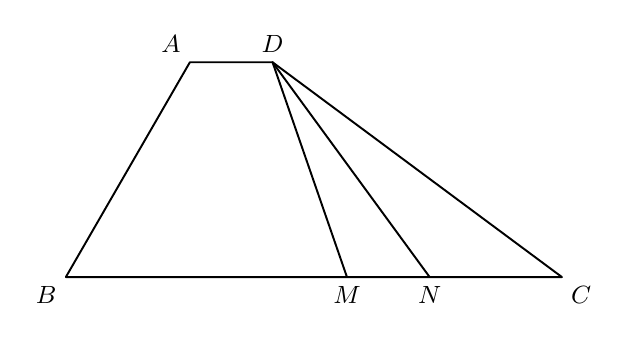
\begin{tikzpicture}[font=\small, line width=0.7pt,
  x=1.05cm, y=1.05cm, line cap=round, line join=round]
  \coordinate (B) at (0,0);
  \coordinate (C) at (6,0);
  \coordinate (A) at (1.5,2.598);
  \coordinate (D) at (2.5,2.598);
  \coordinate (M) at (3.4,0);
  \coordinate (N) at (4.4,0);
  \draw (B)--(C)--(D)--(A)--cycle;
  \draw (D)--(M);
  \draw (D)--(N);
  \node[below left,inner sep=3pt] at (B) {$B$};
  \node[below right,inner sep=3pt] at (C) {$C$};
  \node[above left,inner sep=3pt] at (A) {$A$};
  \node[above,inner sep=3pt] at (D) {$D$};
  \node[below,inner sep=3pt] at (M) {$M$};
  \node[below,inner sep=3pt] at (N) {$N$};
\end{tikzpicture}
\end{center}
\nopagebreak[4]
\end{question}
\gkpart{三、解答题}

\begin{question}
\gkti{16}在 $\triangle ABC$ 中，角 $A$，$B$，$C$ 所对的边分别为 $a$，$b$，$c$。已知 $a=2\sqrt2$，$b=5$，$c=\sqrt{13}$。

（1） 求角 $C$ 的大小；

（2） 求 $\sin A$ 的值；

（3） 求 $\sin\left(2A+\dfrac\pi4\right)$ 的值。

\Needspace{0.4\textheight}
\end{question}
\begin{question}
\gkti{17}如图，在三棱柱 $ABC-A_1B_1C_1$ 中，$CC_1\perp$ 平面 $ABC$，$AC\perp BC$，$AC=BC=2$，$CC_1=3$，点 $D$，$E$ 分别在棱 $AA_1$ 和棱 $CC_1$ 上，且 $AD=1$，$CE=2$，$M$ 为棱 $A_1B_1$ 的中点。

（1） 求证：$C_1M\perp B_1D$；

（2） 求二面角 $B-B_1E-D$ 的正弦值；

（3） 求直线 $AB$ 与平面 $DB_1E$ 所成角的正弦值。
\nopagebreak[4]
\begin{center}% 2020 天津卷 第 17 题：三棱柱 ABC-A1B1C1，D 在 AA1、E 在 CC1、M 为 A1B1 中点
% 来源 PDF：普通高考/2020/2020天津.pdf 第 1 页（A3 横排），印面 1131，第 17 题题干右侧
% 几何按原页矢量数据（单位 pt，y 向下）换算为图面坐标：A(1023.5,666.2)、B(1130.9,638.1)、
%   C(1051.6,638.1)、A1(1023.5,547.1)、B1(1130.9,519.1)、C1(1051.6,519.1)；
%   即顶面 A1B1C1 由底面 ABC 竖直平移得到（侧棱 AA1、BB1、CC1 在图面上等长），
%   与 CC1 ⊥ 平面 ABC 的直棱柱一致。D 在 AA1 上且 AD:DA1 = 1:2，E 在 CC1 上且 CE:EC1 = 2:1，
%   M 为 A1B1 中点。
% 原页线型：实线 AB、AA1、BB1、A1B1、A1C1、C1B1、C1M、B1D；
%   虚线 AC、BC、CC1（被前面 ABB1A1 遮挡）、B1E、DE。
\begin{tikzpicture}[font=\small, line width=0.7pt,
  x=1.75cm, y=1.75cm, line cap=round, line join=round]
  \coordinate (A)  at (0,0);
  \coordinate (B)  at (2.68,0.70);
  \coordinate (C)  at (0.70,0.70);
  \coordinate (A1) at (0,2.98);
  \coordinate (B1) at (2.68,3.68);
  \coordinate (C1) at (0.70,3.68);
  \coordinate (D)  at (0,0.99);
  \coordinate (E)  at (0.70,2.69);
  \coordinate (M)  at ($(A1)!0.5!(B1)$);
  % 可见棱与辅助线
  \draw (A)--(B)--(B1)--(A1)--cycle;
  \draw (A1)--(C1)--(B1);
  \draw (B1)--(D);
  \draw (C1)--(M);
  % 被遮挡的棱与体内线段
  \draw[dashed] (A)--(C)--(B);
  \draw[dashed] (C)--(C1);
  \draw[dashed] (B1)--(E);
  \draw[dashed] (D)--(E);
  % 顶点标注
  \node[below left,inner sep=3pt] at (A) {$A$};
  \node[below right,inner sep=3pt] at (B) {$B$};
  \node[above right,inner sep=3pt] at (C) {$C$};
  \node[left,inner sep=3pt] at (A1) {$A_1$};
  \node[right,inner sep=3pt] at (B1) {$B_1$};
  \node[above,inner sep=2pt] at (C1) {$C_1$};
  \node[left,inner sep=3pt] at (D) {$D$};
  \node[left,inner sep=3pt] at (E) {$E$};
  \node[below,inner sep=2pt] at (M) {$M$};
\end{tikzpicture}
\end{center}
\nopagebreak[4]
\end{question}
\begin{question}
\gkti{18}已知椭圆 $\dfrac{x^2}{a^2}+\dfrac{y^2}{b^2}=1$（$a>b>0$）的一个顶点为 $A(0,-3)$，右焦点为 $F$，且 $|OA|=|OF|$，其中 $O$ 为原点。

（1） 求椭圆方程；

（2） 已知点 $C$ 满足 $3\overrightarrow{OC}=\overrightarrow{OF}$，点 $B$ 在椭圆上（$B$ 异于椭圆的顶点），直线 $AB$ 与以 $C$ 为圆心的圆相切于点 $P$，且 $P$ 为线段 $AB$ 的中点。求直线 $AB$ 的方程。

\end{question}
\begin{question}
\gkti{19}已知 $\{a_n\}$ 为等差数列，$\{b_n\}$ 为等比数列，$a_1=b_1=1$，$a_5=5(a_4-a_3)$，$b_5=4(b_4-b_3)$。

（1） 求 $\{a_n\}$ 和 $\{b_n\}$ 的通项公式；

（2） 记 $\{a_n\}$ 的前 $n$ 项和为 $S_n$，求证：$S_nS_{n+2}<S_{n+1}^2$（$n\in\mathbf N^*$）；

\Needspace{5\baselineskip}
（3） 对任意的正整数 $n$，设
\nopagebreak[4]
\[c_n=\begin{cases}\dfrac{(3a_n-2)b_n}{a_na_{n+2}},&n\text{ \text{为奇数}},\\[2ex]\dfrac{a_{n-1}}{b_{n+1}},&n\text{ \text{为偶数}}.\end{cases}\]
求数列 $\{c_n\}$ 的前 $2n$ 项和。

\end{question}
\begin{question}
\gkti{20}已知函数 $f(x)=x^3+k\ln x$（$k\in\mathbf R$），$f'(x)$ 为 $f(x)$ 的导函数。

（1） 当 $k=6$ 时，

① 求曲线 $y=f(x)$ 在点 $(1,f(1))$ 处的切线方程；

② 求函数 $g(x)=f(x)-f'(x)+\dfrac9x$ 的单调区间和极值；

\Needspace{5\baselineskip}
（2） 当 $k\geqslant-3$ 时，求证：对任意的 $x_1$，$x_2\in[1,+\infty)$，且 $x_1>x_2$，有
\nopagebreak[4]
\[\frac{f'(x_1)+f'(x_2)}{2}>\frac{f(x_1)-f(x_2)}{x_1-x_2}.\]

\end{question}